%% 03.tex
\documentclass[platex,dvipdfmx]{jsreport}

\usepackage{graphicx}
\graphicspath{{./images/}{../images/}}
\usepackage{pdfpages}
\usepackage{tikz}
\usepackage{xcolor}
\definecolor{UD_GREEN}{HTML}{03af7a}
\usepackage{bm}
\usepackage[left=30truemm]{geometry}
\usepackage{amsmath,amssymb}
\numberwithin{equation}{section}



\begin{document}

\chapter{本論}


\section{結果}
\subsection{逆オパール構造}
逆オパール構造に配置されている球の半径0.01ずつを変化させ、ギャップ-ミッドギャップ比の最大化を行った。なお、今回は誘電体媒質の誘電率$\epsilon = 13.0$としてシミュレーションを実行した。
以下に球の半径を変化させていった際のギャップ-ミッドギャップ比の変化を示す。

\begin{figure}[htbp]
  \centering
  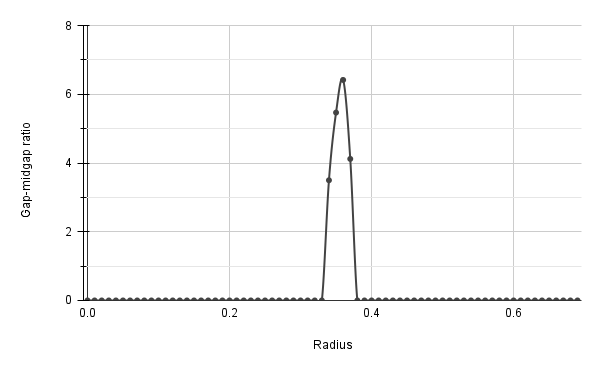
\includegraphics[width=0.8\linewidth]{results/inverse_opals.png}
  \caption{逆オパール構造の球の半径を変化させた際のギャップ-ミッドギャップ比の変化}
  \label{fig:inv_opal}
\end{figure}

$0.34 \leq r / a \leq 0.37$の範囲でのみバンドギャップが確認でき、その中で最大値をとる$r / a = 0.36$のときのギャップ-ミッドギャップ比は最大となりその値は$6.41675 \% $であった。



\subsection{ウッドパイル構造}
ウッドパイル構造中の棒状誘電体の幅を徐々に変化させていった際のギャップ-ミッドギャップ比の変化を示す。

誘電体棒幅$w = 0.28$で最大となり、ギャップ-ミッドギャップ比は$15.17613425 \%$となった。

\subsection{ヤブロノバイト構造}
\section{考察}
\subsection{逆オパール構造}
\subsection{ウッドパイル構造}
\subsection{ヤブロノバイト構造}

\end{document}